\documentclass{beamer}

\usetheme{Szeged}
\usecolortheme{dolphin}

\usepackage[T1]{fontenc}
\usepackage[utf8]{inputenc}
\usepackage{lmodern}
\usepackage{ngerman}
\usepackage{graphicx}
\usepackage{ccicons}

\usepackage{savesym}
\savesymbol{note} % beamer's \note now as \orignote
\usepackage[natbibapa,nodoi]{apacite}
\restoresymbol{apa}{note}% \note now again beamersnote, \apanote is APA \note command

\usepackage{media9}

%
% \AtBeginSection[]
% {
% \begin{frame}
% \tableofcontents[currentsection]
% \end{frame}
% }
%
\setbeamercovered{transparent}

\beamertemplatenavigationsymbolsempty

\title{Sicherer Radfahren}
\subtitle{Wie offene Unfalldaten helfen können}
\author[Dr.\,Thomas Terstiege]{Dr.\,Thomas Terstiege}
\institute[Code for Münster]{Code for Münster}
\date{26. September 2019\\{\scriptsize{}Forum Citizen Science 2019\\		\ccLogo\ccAttribution\ccShareAlike\\
		{\tiny This work is licensed under a Creative Commons Attribution-ShareAlike 4.0 International License (CC BY-SA 4.0).} }}%\\Universität Münster, Institut für Geoinformatik\par}}

\begin{document}

\frame{
  \titlepage
}

\section*{Einleitung}

\begin{frame}
  \frametitle{}
  \framesubtitle{}  
  
  
\includegraphics[width=\textwidth]{img/WN-screenshot.png}
  

  
  \vfill
  {\scriptsize (Bildquelle: \url{https://www.wn.de/Startseite/Startseite-Schattenressort/3673899-Verkehrsunfallstatistik-2018-Ein-schlechter-Tag-fuer-Muenster})\par}
\end{frame}

\subsection{Entwicklung Unfallzahlen}

\begin{frame}
  \frametitle{Entwicklung Unfallzahlen}

  \centering
  
  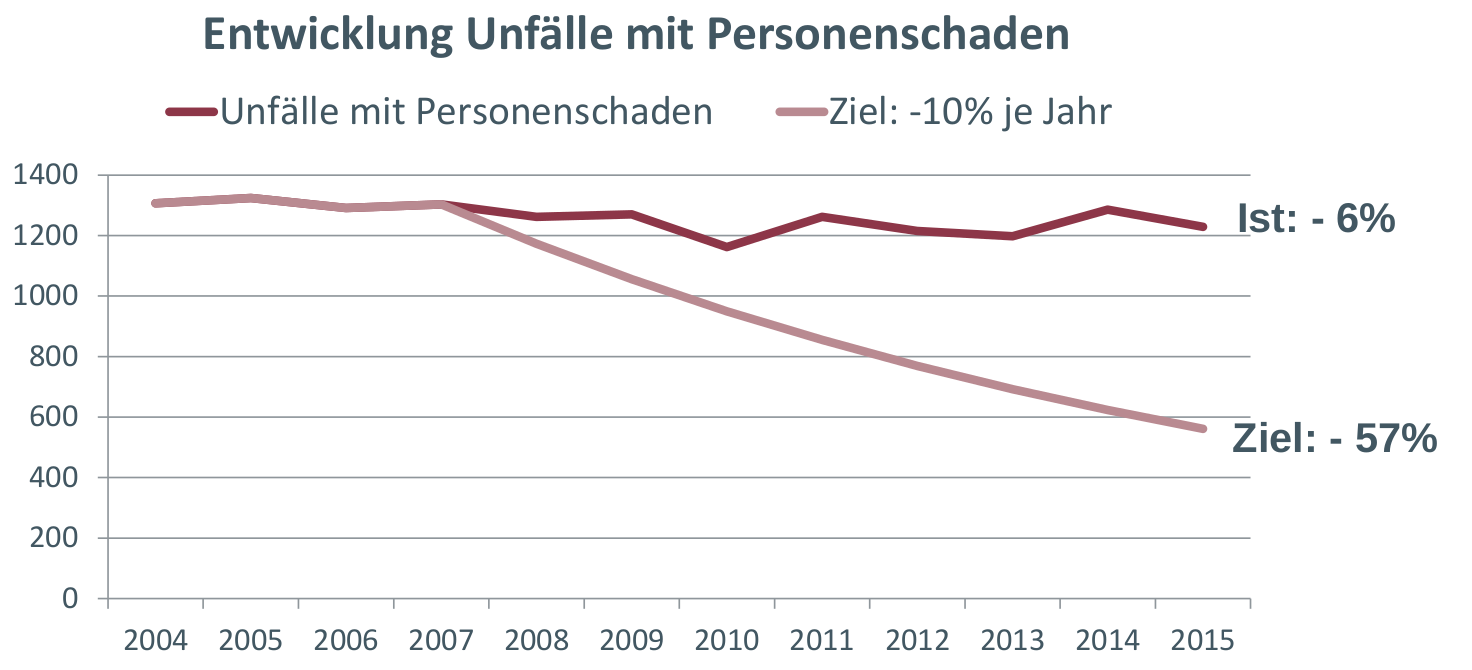
\includegraphics[width=0.9\textwidth]{img/unfaelle-personenschaden-2004-2015.png}
  
  TODO: update with data from 2016-2018, after validating crashes data
  
  % GNUPLOT: LaTeX picture with Postscript
\begingroup
  \makeatletter
  \providecommand\color[2][]{%
    \GenericError{(gnuplot) \space\space\space\@spaces}{%
      Package color not loaded in conjunction with
      terminal option `colourtext'%
    }{See the gnuplot documentation for explanation.%
    }{Either use 'blacktext' in gnuplot or load the package
      color.sty in LaTeX.}%
    \renewcommand\color[2][]{}%
  }%
  \providecommand\includegraphics[2][]{%
    \GenericError{(gnuplot) \space\space\space\@spaces}{%
      Package graphicx or graphics not loaded%
    }{See the gnuplot documentation for explanation.%
    }{The gnuplot epslatex terminal needs graphicx.sty or graphics.sty.}%
    \renewcommand\includegraphics[2][]{}%
  }%
  \providecommand\rotatebox[2]{#2}%
  \@ifundefined{ifGPcolor}{%
    \newif\ifGPcolor
    \GPcolortrue
  }{}%
  \@ifundefined{ifGPblacktext}{%
    \newif\ifGPblacktext
    \GPblacktexttrue
  }{}%
  % define a \g@addto@macro without @ in the name:
  \let\gplgaddtomacro\g@addto@macro
  % define empty templates for all commands taking text:
  \gdef\gplbacktext{}%
  \gdef\gplfronttext{}%
  \makeatother
  \ifGPblacktext
    % no textcolor at all
    \def\colorrgb#1{}%
    \def\colorgray#1{}%
  \else
    % gray or color?
    \ifGPcolor
      \def\colorrgb#1{\color[rgb]{#1}}%
      \def\colorgray#1{\color[gray]{#1}}%
      \expandafter\def\csname LTw\endcsname{\color{white}}%
      \expandafter\def\csname LTb\endcsname{\color{black}}%
      \expandafter\def\csname LTa\endcsname{\color{black}}%
      \expandafter\def\csname LT0\endcsname{\color[rgb]{1,0,0}}%
      \expandafter\def\csname LT1\endcsname{\color[rgb]{0,1,0}}%
      \expandafter\def\csname LT2\endcsname{\color[rgb]{0,0,1}}%
      \expandafter\def\csname LT3\endcsname{\color[rgb]{1,0,1}}%
      \expandafter\def\csname LT4\endcsname{\color[rgb]{0,1,1}}%
      \expandafter\def\csname LT5\endcsname{\color[rgb]{1,1,0}}%
      \expandafter\def\csname LT6\endcsname{\color[rgb]{0,0,0}}%
      \expandafter\def\csname LT7\endcsname{\color[rgb]{1,0.3,0}}%
      \expandafter\def\csname LT8\endcsname{\color[rgb]{0.5,0.5,0.5}}%
    \else
      % gray
      \def\colorrgb#1{\color{black}}%
      \def\colorgray#1{\color[gray]{#1}}%
      \expandafter\def\csname LTw\endcsname{\color{white}}%
      \expandafter\def\csname LTb\endcsname{\color{black}}%
      \expandafter\def\csname LTa\endcsname{\color{black}}%
      \expandafter\def\csname LT0\endcsname{\color{black}}%
      \expandafter\def\csname LT1\endcsname{\color{black}}%
      \expandafter\def\csname LT2\endcsname{\color{black}}%
      \expandafter\def\csname LT3\endcsname{\color{black}}%
      \expandafter\def\csname LT4\endcsname{\color{black}}%
      \expandafter\def\csname LT5\endcsname{\color{black}}%
      \expandafter\def\csname LT6\endcsname{\color{black}}%
      \expandafter\def\csname LT7\endcsname{\color{black}}%
      \expandafter\def\csname LT8\endcsname{\color{black}}%
    \fi
  \fi
    \setlength{\unitlength}{0.0500bp}%
    \ifx\gptboxheight\undefined%
      \newlength{\gptboxheight}%
      \newlength{\gptboxwidth}%
      \newsavebox{\gptboxtext}%
    \fi%
    \setlength{\fboxrule}{0.5pt}%
    \setlength{\fboxsep}{1pt}%
\begin{picture}(7200.00,4320.00)%
    \gplgaddtomacro\gplbacktext{%
      \csname LTb\endcsname%
      \put(747,372){\makebox(0,0)[r]{\strut{}$0$}}%
      \csname LTb\endcsname%
      \put(747,907){\makebox(0,0)[r]{\strut{}$200$}}%
      \csname LTb\endcsname%
      \put(747,1441){\makebox(0,0)[r]{\strut{}$400$}}%
      \csname LTb\endcsname%
      \put(747,1976){\makebox(0,0)[r]{\strut{}$600$}}%
      \csname LTb\endcsname%
      \put(747,2511){\makebox(0,0)[r]{\strut{}$800$}}%
      \csname LTb\endcsname%
      \put(747,3046){\makebox(0,0)[r]{\strut{}$1000$}}%
      \csname LTb\endcsname%
      \put(747,3580){\makebox(0,0)[r]{\strut{}$1200$}}%
      \csname LTb\endcsname%
      \put(747,4115){\makebox(0,0)[r]{\strut{}$1400$}}%
      \csname LTb\endcsname%
      \put(849,186){\makebox(0,0){\strut{}$2004$}}%
      \csname LTb\endcsname%
      \put(1712,186){\makebox(0,0){\strut{}$2006$}}%
      \csname LTb\endcsname%
      \put(2576,186){\makebox(0,0){\strut{}$2008$}}%
      \csname LTb\endcsname%
      \put(3439,186){\makebox(0,0){\strut{}$2010$}}%
      \csname LTb\endcsname%
      \put(4303,186){\makebox(0,0){\strut{}$2012$}}%
      \csname LTb\endcsname%
      \put(5166,186){\makebox(0,0){\strut{}$2014$}}%
      \csname LTb\endcsname%
      \put(6030,186){\makebox(0,0){\strut{}$2016$}}%
      \csname LTb\endcsname%
      \put(6893,186){\makebox(0,0){\strut{}$2018$}}%
    }%
    \gplgaddtomacro\gplfronttext{%
      \csname LTb\endcsname%
      \put(144,2243){\rotatebox{-270}{\makebox(0,0){\strut{}Anzahl Unfälle}}}%
      \csname LTb\endcsname%
      \put(5300,1332){\makebox(0,0)[r]{\strut{}Anzahl Unfälle mit Personenschaden}}%
      \csname LTb\endcsname%
      \put(5300,1146){\makebox(0,0)[r]{\strut{}Ziel Ordnungspartnerschaft (-10\% pro Jahr)}}%
    }%
    \gplbacktext
    \put(0,0){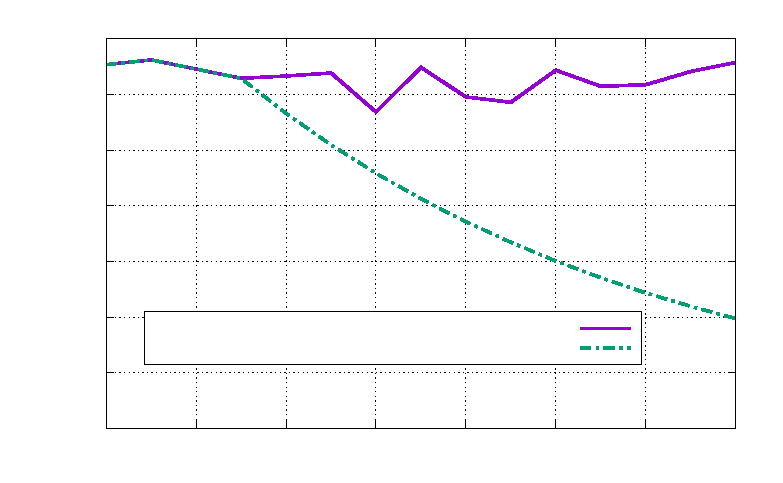
\includegraphics{img/anzahl-unfaelle-pro-jahr}}%
    \gplfronttext
  \end{picture}%
\endgroup

  
    {\scriptsize (Bildquelle: \citealt[Folie~4]{Brockmann2017})\par}
\end{frame}

\begin{frame}
  \frametitle{Entwicklung Unfallzahlen}

  \centering
  
  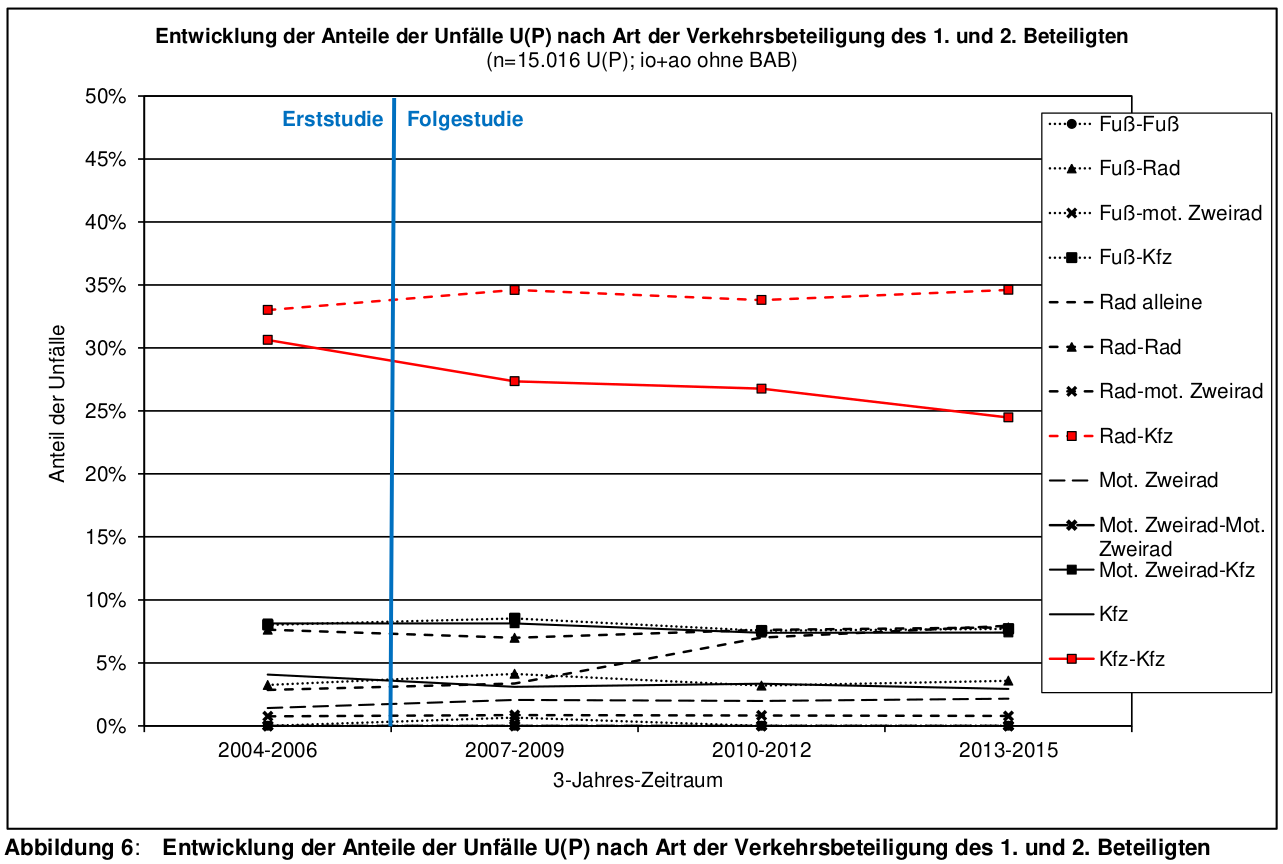
\includegraphics[width=0.925\textwidth]{img/anteil-unfaelle-beteiligte.png}
  
    {\scriptsize (Bildquelle: \citealt[S.~11]{Baier2018})\par}
\end{frame}

\begin{frame}
  \frametitle{Entwicklung Unfallzahlen}

  \centering
  
  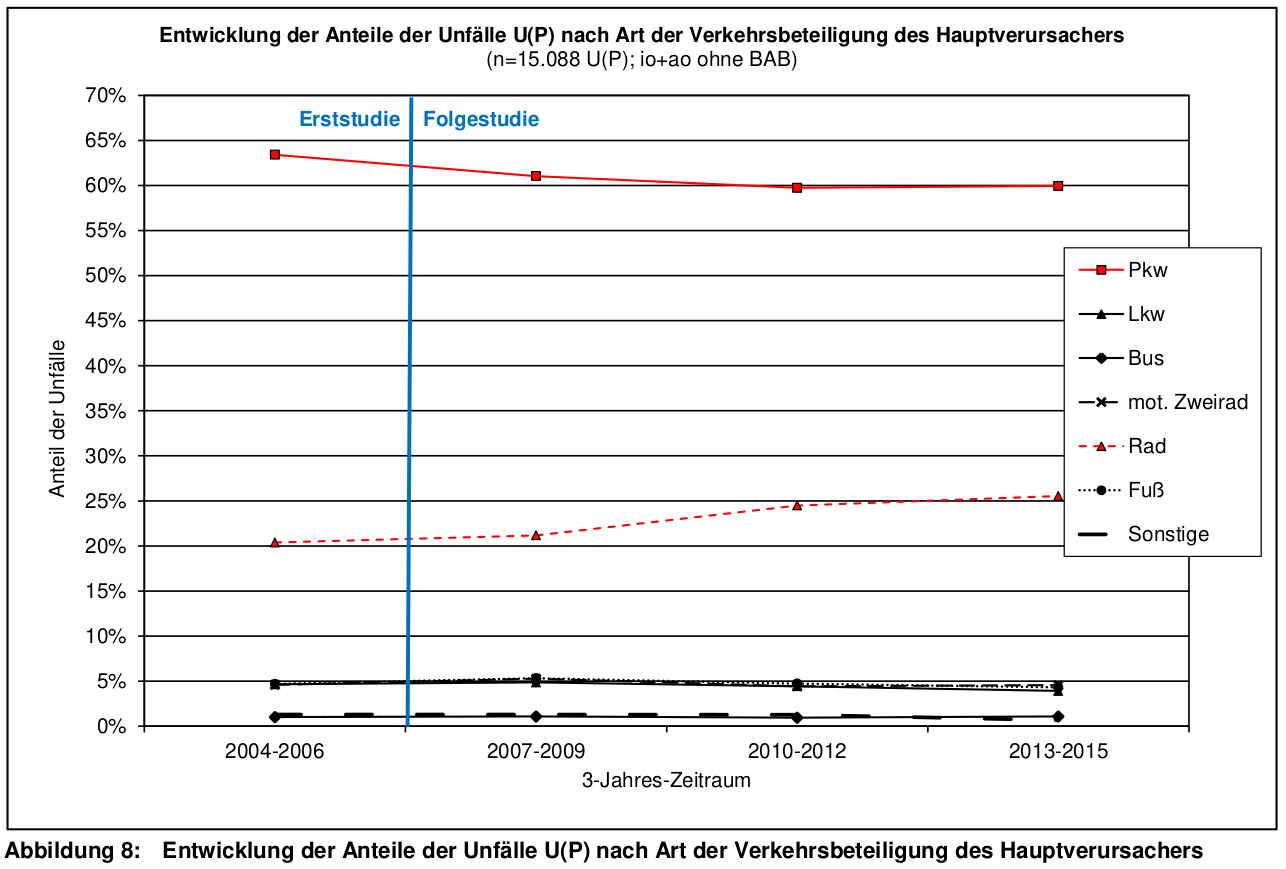
\includegraphics[width=0.925\textwidth]{img/hauptverursacher.png}
  
    {\scriptsize (Bildquelle: \citealt[S.~13]{Baier2018})\par}
\end{frame}


\begin{frame}
  \frametitle{Zugänglichkeit Unfalldaten}
  
  \begin{itemize}
    \item \cite{Polizei2019}: Verkehrsunfallstatistik 2018 der Polizei
    \begin{itemize}
      \item 12 Seiten
      \item hoher Anteil an Rad-Unfällen wird genannt
      \item nur implizit: PKW meist Unfallverursacher
      \item viele Fragen bleiben offen
    \end{itemize}
    \item \cite{Baier2018}: umfangreiche, wichtige Studie
    \item[aber:]
    \begin{itemize}
      \item mehr als 60 Seiten
      \item Kurzfassung 20 Seiten
      \pause
      \item nicht interaktiv
    \end{itemize}    
  \end{itemize}
\end{frame}

\section{Vorstellung "`Crashes"'}



\begin{frame}
  \frametitle{\url{https://crashes.codeformuenster.org}}
  
  \begin{itemize}
    \item Datengrundlage
    \item Rohdaten polizeiliche Verkehrsunfallstatistiken 2007 - 2018
    \begin{itemize}
      \item 
      \item manuelle Ortsangaben
    \end{itemize}
    \item ein Großteil aufwändig geokodiert
  \end{itemize}
  
\end{frame}

\begin{frame}
  \frametitle{\url{https://crashes.codeformuenster.org}}
  
  \href{beispielpraesentation-crashes.mkv}{\url{https://crashes.codeformuenster.org}: Beispielvorführung}
  
\end{frame}

\begin{frame}
  \frametitle{Fahrradstraße?}
  
  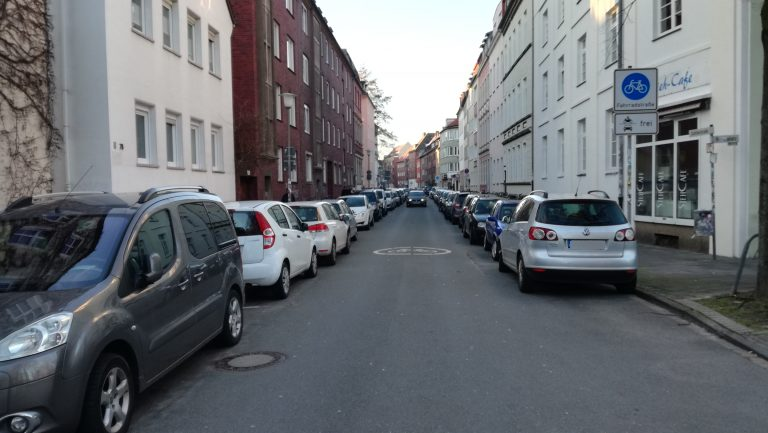
\includegraphics[width=\textwidth]{img/schillerstrasse.jpg}
  
    {\scriptsize (Bildquelle: \url{https://fahrradstadt.ms/2018/02/23/fahrradstrassen-ist-bunt-besser/})\par}
\end{frame}

\begin{frame}
  \frametitle{Details Unfalltypen}
  \centering
  
  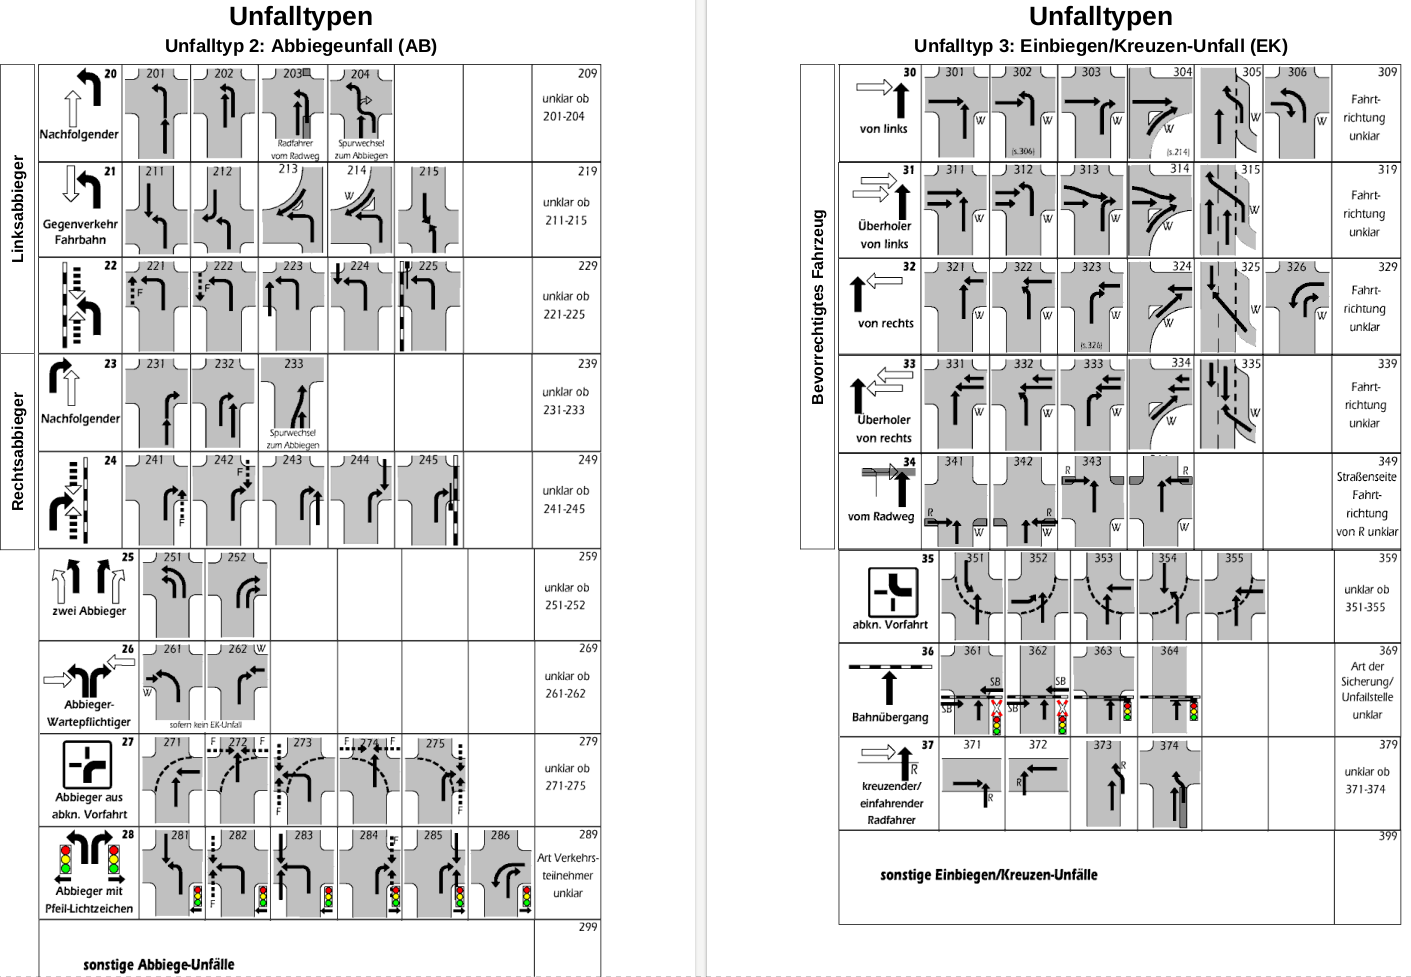
\includegraphics[width=0.9\textwidth]{img/unfalltyp-details.png}
  
  {\scriptsize (Bildquelle: \url{https://recht.nrw.de/lmi/owa/br_show_anlage?p_id=15549})\par}
\end{frame}

\section{Ausblick}

\begin{frame}
  \frametitle{Weitere Schritte}
  
  \centering  
  
  \begin{itemize}
    \item "`Ungenauigkeiten bei der Lokalisierung der Unfälle"' \cite[S.~38]{Baier2018}
    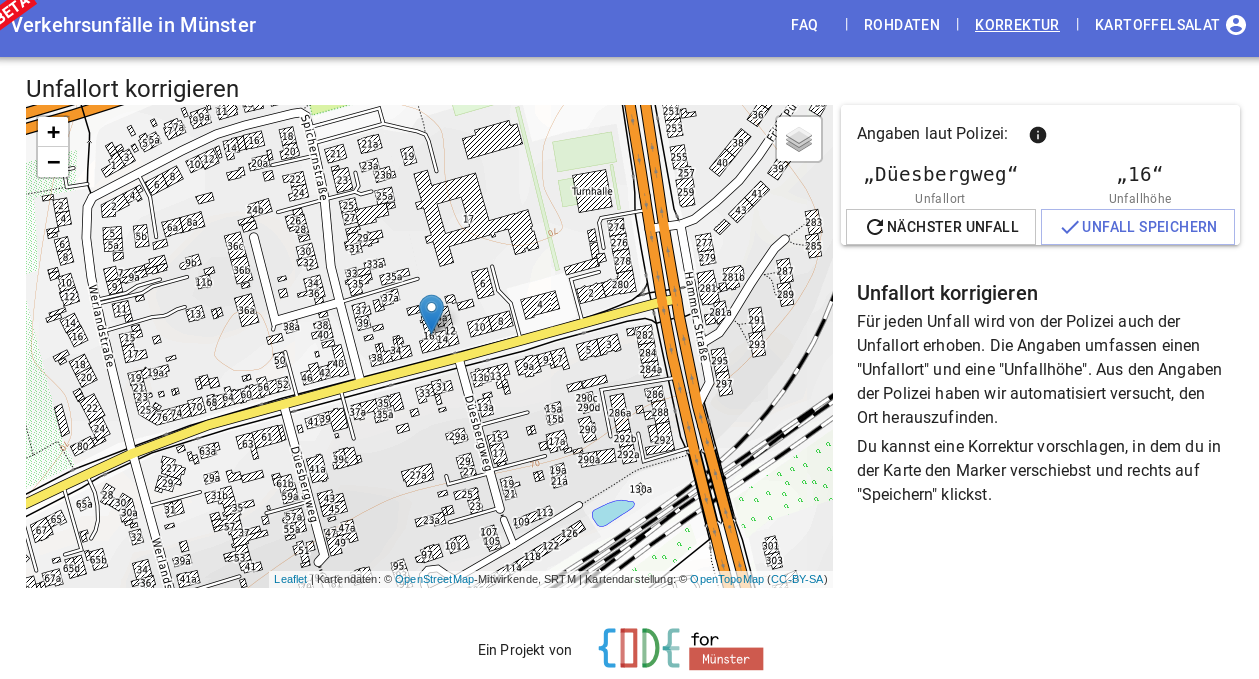
\includegraphics[width=0.8\textwidth]{img/editor-screenshot.png}
    \item filtern nach (vermuteter) Unfallursache
    \item räumlicher Filter
    \item \ldots
  \end{itemize}
\end{frame}

\begin{frame}
  Danke für die Aufmerksamkeit!
  
  Besonderen Dank an:

\end{frame}

\section{Literaturverzeichnis}
\begin{frame}[plain]%[allowframebreaks]
  \frametitle{\secname{}} %\insertcontinuationcount}
% 	\vspace*{0.35cm}
	\begin{center}
		\LARGE\textbf{Vielen Dank!}
	\end{center}
	
%  	\setlength{\linewidth}{1.085\linewidth}
% 	\vspace*{-0.4cm}
%   \textbf{\footnotesize References}
%   \renewcommand\bibliographytypesize{\fontsize{4}{4}\selectfont}
	\bibliographystyle{apacite}	
	\bibliography{references}
\end{frame}

\newcounter{finalframe}
\setcounter{finalframe}{\value{framenumber}}
\appendix
\begin{frame}[allowframebreaks,fragile]
\end{frame}
\setcounter{framenumber}{\value{finalframe}}
\end{document}
